\documentclass[apj]{aastex62}
\shorttitle{Delay Time Distributions of SNe~Ia}
\shortauthors{Strolger et al.}

\usepackage{natbib}
\usepackage{nicefrac}
\usepackage{ulem}
\usepackage{xcolor}
\usepackage{topcapt}
\usepackage{amssymb,amsmath}
\bibliographystyle{aasjournal}

\renewcommand{\deg}{^{\circ}}
\begin{document}
\title{The Empirical Delay Time Distributions of Type Ia Supernovae From Galaxy and Cosmic Star Formation Histories}
\author[0000-0002-7756-4440]{L.-G.~Strolger}
\author{Steven Rodney}
\author{Camila Pacifici}
\author{et al.}

\begin{abstract}
\textcolor{red}{blah, blah, blah \ldots}
\end{abstract}

\section{Introduction}
Understanding cosmic type Ia supernova (SN~Ia) rates have a critical importance to understanding galaxy evolutionary feedback mechanisms, the cosmic iron enrichment and $\alpha$-process element enrichment histories \citep{Maoz:2017ck}, and constraining the physical mechanisms of SN~Ia progenitors. However, tracing rate histories has been a slog, with the first precise measures of the local ($z\approx0.0$) rate in the early 1990s \cite[cf.][]{Cappellaro:1993qm,Cappellaro:1997,Cappellaro:1999}, and the first measures beyond the local Hubble flow beginning in the early 2000s as collateral results of the dark energy experiments~\citep{Riess:1998,Perlmutter:1999}. Since then, there have been several measures of the volumetric SN~Ia rate at various redshifts by various groups. These rate values have not always been in total agreement with one another, and there may be several valid reasons as to why (see rev. by \textcolor{red}{Haden?}). For the time being, it is probably best to consider each published rate as a valid measure that may (or may not) have misestimated uncertainties. A collection of those volumetric SN~Ia rates is shown in Table~\ref{tab:sn1a_rates} and Figure~\ref{fig:sn1a_rates}.  For illustration, we bin the rate data into 8 quantiles of nearly equal number of measures, and present those binned measures, weighted by reported statistical uncertainties only, in Table~\ref{tab:sn1a_bin} and Figure~\ref{fig:sn1a_rates}.

\begin{figure}[t]
   \centering
   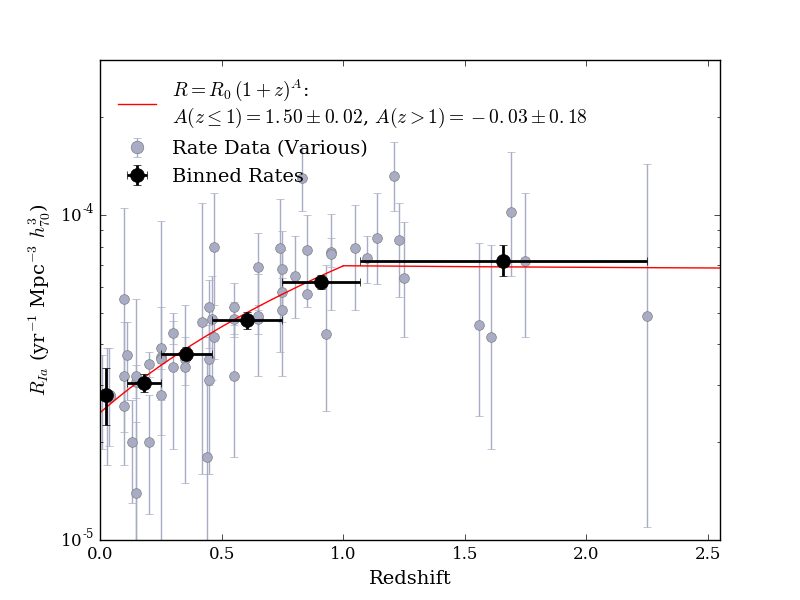
\includegraphics[width=6.1in]{figure_SNIa_rate_z_pwr_fit}
   \caption{\footnotesize Type Ia supernova volumetric rate measures from various sources in the literature (gray points, see Table~\ref{tab:sn1a_rates} for their sources), and binned (black points, see Table~\ref{tab:sn1a_bin}), largely for illustration. The solid red lines show a broken power-law fit to the data in redshift space. The dashed red line (and associated uncertainty region, in gray) is from~\cite{Okumura:2014}.}
   \label{fig:sn1a_rates}
\end{figure}


\startlongtable
\begin{deluxetable}{lcccl}
\tablecaption{Volumetric SN Ia Rates Used in this Work}
\tablehead{
\colhead{Redshift} & \colhead{$R_{\rm Ia}$\tablenotemark{a}} &\colhead{Stat. Uncertainty} & \colhead{Sys. Uncertainty} & \colhead{Source}}

\startdata
0.01&0.28&$^{+0.09}_{-0.09}$&$^{+0.0}_{-0.0}$&\cite{Cappellaro:1999}\\
0.03&0.28&$^{+0.11}_{-0.11}$&$^{+0.0}_{-0.0}$&\cite{Mannucci:2005}\\
0.0375&0.278&$^{+0.112}_{-0.083}$&$^{+0.015}_{-0.00}$&\cite{Dilday:2010}\\
0.1&0.259&$^{+0.052}_{-0.044}$&$^{+0.028}_{-0.001}$&\cite{Dilday:2010}\\
0.10&0.32&$^{+0.15}_{-0.15}$&$^{+0.0}_{-0.0}$&\cite{Madgwick:2003}\\
0.10&0.55&$^{+0.50}_{-0.29}$&$^{+0.20}_{-0.20}$&\cite{Cappellaro:2015oq}\\
0.11&0.37&$^{+0.10}_{-0.10}$&$^{+0.0}_{-0.0}$&\cite{strolger2003}\\
0.13&0.20&$^{+0.07}_{-0.07}$&$^{+0.05}_{-0.05}$&\cite{Blanc:2004}\\
0.15&0.307&$^{+0.038}_{-0.034}$&$^{+0.035}_{-0.005}$&\cite{Dilday:2010}\\
0.15&0.32&$^{+0.23}_{-0.23}$&$^{+0.23}_{-0.06}$&\cite{Rodney:2010b}\\
0.16&0.14&$^{+0.09}_{-0.09}$&$^{+0.06}_{-0.12}$&\cite{Perrett:2012}\\
0.2&0.348&$^{+0.032}_{-0.030}$&$^{+0.082}_{-0.007}$&\cite{Dilday:2010}\\
0.20&0.20&$^{+0.08}_{-0.08}$&$^{+0.0}_{-0.0}$&\cite{Horesh:2008}\\
0.25&0.36&$^{+0.60}_{-0.26}$&$^{+0.12}_{-0.35}$&\cite{Rodney:2014fj}\\
0.25&0.365&$^{+0.031}_{-0.028}$&$^{+0.182}_{-0.012}$&\cite{Dilday:2010}\\
0.25&0.39&$^{+0.13}_{-0.12}$&$^{+0.10}_{-0.10}$&\cite{Cappellaro:2015oq}\\
0.26&0.28&$^{+0.07}_{-0.07}$&$^{+0.06}_{-0.07}$&\cite{Perrett:2012}\\
0.30&0.34&$^{+0.16}_{-0.15}$&$^{+0.0}_{-0.0}$&\cite{Botticella:2008}\\
0.30&0.434&$^{+0.037}_{-0.034}$&$^{+0.396}_{-0.016}$&\cite{Dilday:2010}\\
0.35&0.34&$^{+0.19}_{-0.19}$&$^{+0.19}_{-0.03}$&\cite{Rodney:2010b}\\
0.35&0.36&$^{+0.06}_{-0.06}$&$^{+0.05}_{-0.06}$&\cite{Perrett:2012}\\
0.42&0.46&$^{+0.42}_{-0.32}$&$^{+ 0.10}_{-0.13}$&\cite{Graur:2014}\\
0.44&0.262&$^{+ 0.229}_{-0.133}$&$^{+ 0.059}_{-0.120}$&\cite{Okumura:2014}\\
0.45&0.31&$^{+0.15}_{-0.15}$&$^{+0.15}_{-0.04}$&\cite{Rodney:2010b}\\
0.45&0.36&$^{+0.06}_{-0.06}$&$^{+0.04}_{-0.05}$&\cite{Perrett:2012}\\
0.45&0.52&$^{+0.11}_{-0.13}$&$^{+0.16}_{-0.16}$&\cite{Cappellaro:2015oq}\\
0.46&0.48&$^{+0.17}_{-0.17}$&$^{+0.0}_{-0.0}$&\cite{Tonry:2003}\\
0.47&0.42&$^{+0.06}_{-0.06}$&$^{+0.13}_{-0.09}$&\cite{Neill:2006}\\
0.47&0.80&$^{+0.37}_{-0.27}$&$^{+1.66}_{-0.26}$&\cite{Dahlen:2008}\\
0.55&0.32&$^{+0.14}_{-0.14}$&$^{+0.14}_{-0.07}$&\cite{Rodney:2010b}\\
0.55&0.48&$^{+0.06}_{-0.06}$&$^{+0.04}_{-0.05}$&\cite{Perrett:2012}\\
0.55&0.52&$^{+0.10}_{-0.09}$&$^{+0.0}_{-0.0}$&\cite{Pain:2002}\\
0.65&0.48&$^{+0.05}_{-0.05}$&$^{+0.04}_{-0.06}$&\cite{Perrett:2012}\\
0.65&0.49&$^{+0.17}_{-0.17}$&$^{+0.17}_{-0.08}$&\cite{Rodney:2010b}\\
0.65&0.69&$^{+0.19}_{-0.18}$&$^{+0.27}_{-0.27}$&\cite{Cappellaro:2015oq}\\
0.74&0.79&$^{+0.33}_{-0.41}$&$^{+0.0}_{-0.0}$&\cite{Graur:2011}\\
0.75&0.51&$^{+0.27}_{-0.19}$&$^{+0.23}_{-0.19}$&\cite{Rodney:2014fj}\\
0.75&0.58&$^{+0.06}_{-0.06}$&$^{+0.05}_{-0.07}$&\cite{Perrett:2012}\\
0.75&0.68&$^{+0.21}_{-0.21}$&$^{+0.21}_{-0.14}$&\cite{Rodney:2010b}\\
0.80&0.839&$^{+ 0.230}_{-0.185}$&$^{+ 0.060}_{-0.120}$&\cite{Okumura:2014}\\
0.83&1.30&$^{+0.33}_{-0.27}$&$^{+0.73}_{-0.51}$&\cite{Dahlen:2008}\\
0.85&0.57&$^{+0.05}_{-0.05}$&$^{+0.06}_{-0.07}$&\cite{Perrett:2012}\\
0.85&0.78&$^{+0.22}_{-0.22}$&$^{+0.22}_{-0.16}$&\cite{Rodney:2010b}\\
0.94&0.45&$^{+0.22}_{-0.19}$&$^{+ 0.13}_{-0.06}$&\cite{Graur:2014}\\
0.95&0.76&$^{+0.25}_{-0.25}$&$^{+0.25}_{-0.26}$&\cite{Rodney:2010b}\\
0.95&0.77&$^{+0.08}_{-0.08}$&$^{+0.10}_{-0.12}$&\cite{Perrett:2012}\\
1.05&0.79&$^{+0.28}_{-0.28}$&$^{+0.28}_{-0.41}$&\cite{Rodney:2010b}\\
1.1&0.74&$^{+0.12}_{-0.12}$&$^{+0.10}_{-0.13}$&\cite{Perrett:2012}\\
1.14&0.705&$^{+ 0.239}_{-0.183}$&$^{+ 0.102}_{-0.103}$&\cite{Okumura:2014}\\
1.21&1.32&$^{+0.36}_{-0.29}$&$^{+0.38}_{-0.32}$&\cite{Dahlen:2008}\\
1.23&0.84&$^{+0.25}_{-0.28}$&$^{+0.0}_{-0.0}$&\cite{Graur:2011}\\
1.25&0.64&$^{+0.31}_{-0.22}$&$^{+0.34}_{-0.23}$&\cite{Rodney:2014fj}\\
1.59&0.45&$^{+0.34}_{-0.22}$&$^{+ 0.05}_{-0.09}$&\cite{Graur:2014}\\
1.61&0.42&$^{+0.39}_{-0.23}$&$^{+0.19}_{-0.14}$&\cite{Dahlen:2008}\\
1.69&1.02&$^{+0.54}_{-0.37}$&$^{+0.0}_{-0.0}$&\cite{Graur:2011}\\
1.75&0.72&$^{+0.45}_{-0.30}$&$^{+0.50}_{-0.28}$&\cite{Rodney:2014fj}\\
2.25&0.49&$^{+0.95}_{-0.38}$&$^{+0.45}_{-0.24}$&\cite{Rodney:2014fj}\\
\enddata
\tablenotetext{a}{In units $10^{-4}$ yr$^{-1}$ Mpc$^{-3}$ $h_{70}^3$}
\label{tab:sn1a_rates}
\end{deluxetable}

It would be reasonable to assume the volumetric rates follow a broken power law evolution with redshift, i.e., $R_{\rm Ia}=R_0\,(1+z)^A$ where at $z<1$ the power-law slope is $A=1.50\pm0.02$ (with $R_0 = 2.47\pm0.02\times10^{-5}$ yr$^{-1}$ Mpc$^{-3}$ $h_{70}^3$), which flattens substantially to $A=-0.06\pm0.2$ at redshifts greater than 1, as is shown in  Figure~\ref{fig:sn1a_rates}. This is broadly consistent with the power-law fit of \cite{Okumura:2014}, especially to $z\sim1$, and the locus is consistent with the volumetric SN~Ia rate at $z\approx0$ converted by \cite{Li:2011b} to $2.7\pm0.3\times10^{-5}$ yr$^{-1}$. 

\begin{table}[h]
   \centering
   \caption{Binned volumetric SN~Ia rates, with statistical uncertainties.}
   \begin{tabular}{lcc} 
   \hline
   \hline
   Redshift & $R_{\rm Ia}$\tablenotemark{a}&N$_{\rm measures}$\\
   \hline
$0.07 \pm{0.06}$ & $0.28^{+0.04}_{-0.03}$& 7\\
$0.19 \pm{0.06}$ & $0.30^{+0.02}_{-0.02}$& 6\\
$0.33 \pm{0.08}$ & $0.38^{+0.02}_{-0.02}$& 8\\
$0.44 \pm{0.03}$ & $0.35^{+0.05}_{-0.04}$& 6\\
$0.61 \pm{0.14}$ & $0.47^{+0.03}_{-0.03}$& 9\\
$0.81 \pm{0.07}$ & $0.60^{+0.04}_{-0.04}$& 7\\
$1.05 \pm{0.17}$ & $0.76^{+0.06}_{-0.06}$& 7\\
$1.73 \pm{0.52}$ & $0.61^{+0.14}_{-0.10}$& 7\\
\hline
   \end{tabular}
   \tablenotetext{a}{In units $10^{-4}$ yr$^{-1}$ Mpc$^{-3}$ $h_{70}^3$}
   \label{tab:sn1a_bin}
\end{table}


While the broken power-law model is useful for predicting yields from volumetric surveys, e.g., for the Wide Field InfraRed Survey Telescope \cite[\textit{WFIRST, }][]{Hounsell:2018fv}, it does not inherently reveal much on the nature of SN~Ia progenitor mechanisms. This is better done through an assessment of delay-time distributions.


\section{Delay Time Distributions from Volumetric SN~Ia Rates and the Cosmic Star Formation History}

For these types of analyses, the standard assumption is that the stellar death rate (or supernova rate) is related to the stellar birth rate, convolved with some delay-time distribution that contains all the temporal factors of stellar evolution (e.g., main sequence lifetime, etc.) and binary star evolution (e.g., accretion rates or merger times). Two additional terms include the fraction of the initial mass function (or IMF) that are the progenitors to the SNe~Ia (presumably $3 - 8\, \rm{M}_{\odot}$ zero-age main sequence stars, see discussion in Section~\ref{sec:wds}), and the fraction of that population that are actually capable of producing events, as not are necessarily in the right type of binary system or systems.

We can relate volumetric SN~Ia rate history to the cosmic star formation history($\dot{\rho}_{\star}$) in a similar way, expressed mathematically by, 
\begin{equation}
R_{\rm Ia}(t) =  h^2\,k\,\varepsilon\,\biggl[\dot{\rho}_{\star}(t) \ast \Phi(t)\biggr],
\label{eqn:std}
\end{equation}
\noindent where $\Phi(t)$ is the delay-time distribution of SNe~Ia, $k$ is the fraction of the IMF (by mass) responsible for SN~Ia progenitors, $\varepsilon$ is the fraction of that population that are ultimately successful in producing SNe~Ia, and $t$ is the forward-moving clock of the universe. 

\subsection{The Fraction of Stars Responsible for SNe~Ia}~\label{sec:wds}
Dissecting each of these terms, $k$ is perhaps the easiest to approximate. The progenitors of SNe~Ia have traditionally been CO WD which acquire sufficient mass to approach or exceed the Chandrasekhar mass limit, $M_{ch}=1.44\,M_{\odot}$. To only marginally achieve this, they can either start at sufficiently high mass to require only a small amount of accretion from a nearby companion (typically single-degenerate, or SD, scenarios), or as a pair of WD that have combined in mass to meet this criterion (the double-degenerate, or DD, scenario) setting an even lower constraint~\cite[see][ for a review]{Maoz:2013}. In the case of WD/WD mergers, WD mass distributions are strongly peaked around $M_{\rm WD}\approx0.6\pm0.1\,M_{\odot}$ \citep{Catalan:2008il}, in which a pair drawn from such distribution may be satisfactorily close to the ignition threshold of a carbon core for a non-rotating CO WD, approximately $1.38\, M_{\odot}$ \citep{Arnett:1969dw, Nomoto:1982vh}. Initial-Final Mass relations \cite[e.g.,][]{Catalan:2008il,Cummings:2018oe} would correspond these to zero-age main-sequence (ZAMS) masses of approximately $3\, M_{\odot}$, but no less than approximately $2.5\, M_{\odot}$. 

The same Initial-Final Mass relations would suggest that a WD essentially at $M_{ch}$ would fall just below $8\, M_{\odot}$ ZAMS. On a more physical bases, simulations show that the lowest mass in which C ignition is still possible is around $6-8 \,M_{\odot}$~\cite{Chen:2014rb,Denissenkov:2015rf}, but likely no more than $\sim11\, M_{\odot}$ \citep{Takahashi:2013jx}, above which an electron-capture-induced collapse mechanism begins, marking the onset of core-collapse supernovae.

It is reasonable, therefore, to assume a progenitor mass range of about $3-8\,M_{\odot}$ ZAMS. From a numerical assessment of these stars, assuming they fall within an IMF that is a power-law distribution by mass (in this initial mass range) with $\alpha\approx-2.3$~\citep{Salpeter:1955rw,Kroupa:2001gf}, one would expect 
\begin{equation}
k = \frac{\int\limits_{3M_{\odot}}^{8M_{\odot}} \xi(M)\,dM}{\int\limits_{0.1M_{\odot}}^{125M_{\odot}} M\,\xi(M)\,dM},
\end{equation}
\noindent where $k = 0.021^{+33\%}_{-24\%}\,M_{\odot}^{-1}$. The error in $k$ is driven more by choices in the upper and lower value in the selected mass range of SN~Ia progenitors than by the choice in IMF model, as detailed above.

The fraction of CO WDs that are successful in making SNe~Ia is hard to determine, as we do not quite yet know the details of the progenitor mechanism or mechanisms. Estimates swing rather wildly from (perhaps) from as low as 1 in 200~\citep{Breedt:2017rp} to as optimistic as 1 in 40~\citep{Maoz:2012}. There is at least strong consensus that accretion on to a CO WD is essential, but very different plausible WD close binary scenarios from at least a theoretical standpoint~\citep{Nelemans:2001hb,Nelemans:2001cs}. The binary fractions of WDs has been recently estimated from the  the ESO-VLT Supernova-Ia Progenitor Survey~\citep[ SPY]{Napiwotzki:2007} show close double WD systems may have $\varepsilon_{\rm bin}\simeq0.1\pm0.02$, with separations distributed following a power-law slope of $\alpha=-1.3\pm0.2$~\citep{Maoz:2017zl}. It is not likely all of these successfully yield SNe~Ia as their merger rates in the MW are at least a magnitude higher than best estimates of the SN~Ia rate in our galaxy, and presumably some of these will form AM CVn and R~Corona Borealis stars, but at least it could be treated as an upper limit on $\varepsilon$.

\subsection{The Star Formation Density History}
The cosmic star formation history (CSFH), at least to $z < 5$, or over 90\% of the history of the universe, is fairly well understood, with~\cite[][ MD14 hereafter]{Madau:2014fk} providing one of the most complete compilations. More recently, the CSFH derived from the combined GAMA, G10-COSMOS, and 3D-HST datasets by~\cite{Driver:2018nr}, in a quasi-homogeneous analysis over a larger area, provides a dataset with greatly reduced uncertainties per datum, but fewer data than shown in the MD14 compendium (see Figure~\ref{fig:csfhs}).  We combine the MD14 and \cite{Driver:2018nr} data, with additional star-formation rate densities from \cite{Bouwens:2015qy} and \cite{Khusanova:2019kx}, to arrive at todays compendium CSFH using the parameterization,
\begin{equation}
\dot{\rho}_{\star}(z) = \frac{A\,(1+z)^C}{((1+z)/B)^D+1}.\label{eqn:mdp}
\end{equation}

\begin{figure}[b]
   \centering
   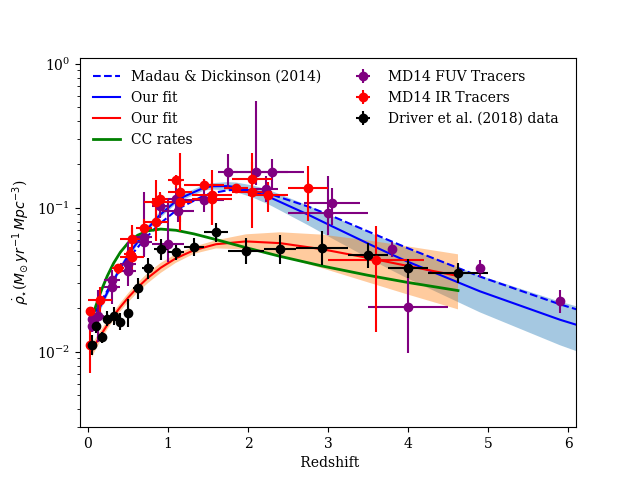
\includegraphics[width=6.1in]{figure_csfh_today}
   \caption{\footnotesize Shown are a compendium of cosmic star formation histories, from ~\cite{Madau:2014fk}, \cite{Driver:2018nr}, \cite{Bouwens:2015qy}, and \cite{Khusanova:2019kx}. Dashed lines (and associated shaded regions) are previous models  from \cite{Madau:2014fk}, \cite{Finkelstein:2014fj}, \cite{Strolger:2015aa}, as indicated. Solid blue line (and blue shaded region) represent our best-fit model to the compendium of data.}
   \label{fig:csfhs}
\end{figure}

\begin{table}[h]
    \centering
    \caption{Cosmic Star Formation History Parameter Fits}
    \label{tab:csfh_fits}
    \begin{tabular}{lcccc}
         & $A$ & $B$ & $C$ & $D$ \\
        \hline
        \hline
	\cite{Madau:2014fk} only & $0.013 \pm 0.001$ & $2.6 \pm 0.1$ & $3.2 \pm 0.2$ & $6.1 \pm 0.2$\\
	\cite{Driver:2018nr}\tablenotemark{a} only & $0.014 \pm 0.001$ & $2.5 \pm 0.2$ & $3.3 \pm 0.3$ & $6.2 \pm 0.3$\\
	\hline
	All Combined Data & $0.0134 \pm 0.0009$ & $2.55 \pm 0.09$ & $3.3 \pm 0.2$ & $6.1 \pm 0.2$\\
	\hline
    \end{tabular}
    \tablenotetext{a}{Corrected for dust attenuation.}
\end{table}

To do so, we must correct the \cite{Driver:2018nr} data for dust attenuation following the prescription in MD14, by applying 
\begin{equation}
	\dot{\rho}_{\star}(z) =h^3\,\biggl[1+10^{0.4\cdot A_{\rm FUV}(z)}\biggr]\, \dot{\rho}_{\star, {\rm uncorrected}}(z),
\end{equation}
where it is assumed $A_{\rm FUV}(z)$ has essentially the same functional form of Equation~\ref{eqn:mdp}, and when applied to the MD14 $A_{\rm FUV}(z)$ data results in a Levenberg-Marquardt least-squares solution of $A=1.4\pm0.1$, $B=3.5\pm0.4$, $C=0.7\pm0.2$, and $D=4.3\pm0.7$. We then fit Equation~\ref{eqn:mdp} to the combined CSFH datasets,    resulting in parameters which are shown in Table~\ref{tab:csfh_fits} and Figure~\ref{fig:csfhs}. 



\subsection{SN~Ia Progenitor Delay-Time Distribution Models}
\noindent \textcolor{red}{Talk about the expected delay-time distribution, values from Graur and Maoz, inability to probe beyond turnover at `SN high noon', around $z\sim1$}. Power law models are defined as $\Phi(t)=t^{\beta}$\ldots

\begin{figure}[b]
   \centering
   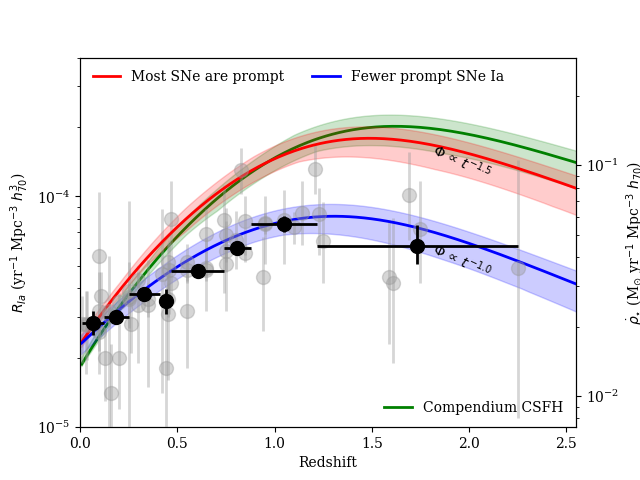
\includegraphics[width=6.5in]{figure_SNIa_rate_alpha}
   \caption{\footnotesize Shown in comparison to the data from Figure~\ref{fig:sn1a_rates} are the expected volumetric rates for power-law delay-time distributions ($\alpha = 1.0$ and 1.5 in red and blue, respectively) as applied to the compendium CSFH (in green and second ordinate). \textcolor{red}{Something about scaling, N/M or fraction}. Smaller $\alpha$ models require a higher fraction of WD progenitors.}
   \label{fig:sn1a_rates2}
\end{figure}

Following the methodology in \cite{Strolger:2010}, we can continue to test a more robust delay-time model, capable of reproducing the theoretical distributions for SD and DD models at one extreme, and $\delta$-function delay times at the other. The unimodal, skew-normal $\Phi(\tau)$ function is defined as:

\begin{equation}
	\Phi(\tau)=\frac{1}{\omega\pi}\,\exp\biggl(\frac{-(\tau-\xi)^2}{2\omega^2}\biggr)\int_{-\infty}^{\alpha (\frac{\tau-\xi}{\omega})} \exp\biggl(\frac{-t'^2}{2}\biggr)\,dt',
\label{eqn:model}
\end{equation}

\noindent where location ($\xi$),\footnote{Different from the initial mass function, $\xi(M)$.} width ($\omega^2$), and shape ($\alpha$)\footnote{Different from the initial mass function power-law slope at the low-mass end.} are defined by the model. Figure~\ref{fig:dtd_families} demonstrates the flexibility of the model in producing various distributions in $\tau$. Either through and optimized fit of the model parameters, or through a Markov-chain monte carlo (MCMC), we can test model $\Phi(\tau)$ through Equation~\ref{eqn:std} in comparison to the volumetric rate measurements.

\begin{figure}[t]
   \centering
   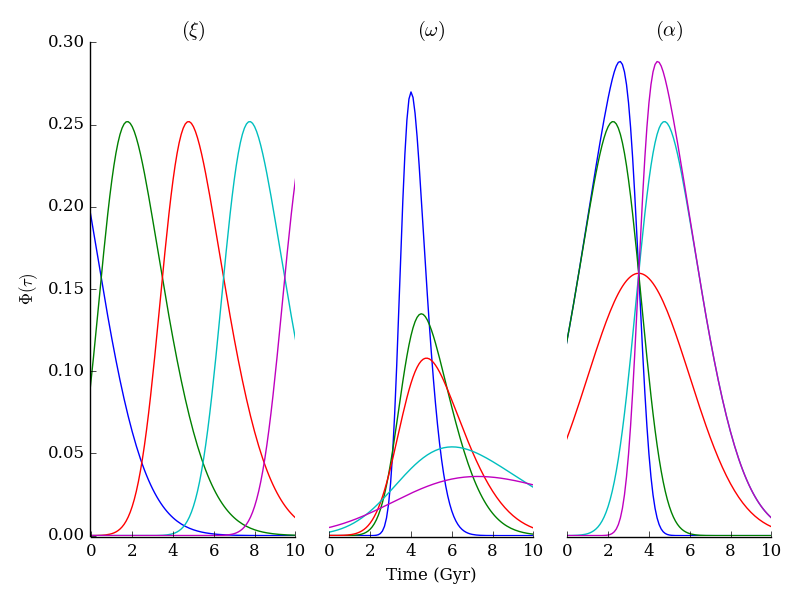
\includegraphics[width=4in]{figure_dtd_families}
   \caption{\footnotesize Families of delay-time distributions models shown for various values of location ($\xi$) fixing other parameters (left plot of figure), width ($\omega$, middle plot), and shape ($\alpha$, right plot), for illustration purposes.}
   \label{fig:dtd_families}
\end{figure}


\subsection{The Optimized Solution\label{sec:optimized_soln}}
We apply a maximum likelihood estimation method to determine the best-fit unimodal delay time model to Equation~\ref{eqn:std} using a method described in \cite{Hogg:2010fj} and the {\tt emcee.py} documentation~\citep{Foreman-Mackey:2013pd}. We assume, for simplicity, that the errors of all survey data are gaussian in nature, but may be underestimated by some factor ($f$), which may be correctly justified given we are only using the statistical error reported for each value.  As follows, we adopt the likelihood function to be:
\begin{equation}
\ln p(y|x, \sigma, \varepsilon, \xi, \omega, \alpha, f) = -\frac{1}{2} \sum_i \biggl\{ \frac{[R_{{\rm Ia},i} - R_{\rm Ia}(t_i; \varepsilon, \xi, \omega, \alpha)]^2}{s_i^2}+\ln (2\pi s_i^2)\biggr\},
	\label{eqn:lf}
\end{equation}
where,
\begin{equation}
s_i^2 = \sigma_i^2+f^2\, R_{\rm Ia}(t_i; \varepsilon, \xi, \omega, \alpha)^2,
\end{equation}
\noindent $R_{{\rm Ia},i}$ are the various rate measures, and $R_{\rm Ia}(t_i)$ are the parameter-dependent model predictions at the cosmic time of the various rate measures. We then find the optimal parameters which maximize this likelihood. As for priors, we require the successful fraction of progenitors to be between zero and unity ($0<\varepsilon<1$), that the width parameter can only be positive ($\omega>0$), and the that underestimation fraction can only be between approximately zero and unity ($-4<\ln f<0$). Otherwise, we apply rather loose and arbitrarty bounds of $-2000<\xi<2000$ and  $-500 < \alpha < 500$. The results of this fit are shown in Figure~\ref{fig:sfd_optimized_curvefit} and Table~\ref{tab:results}. 

\begin{figure}[t] %  figure placement: here, top, bottom, or page
   \centering
   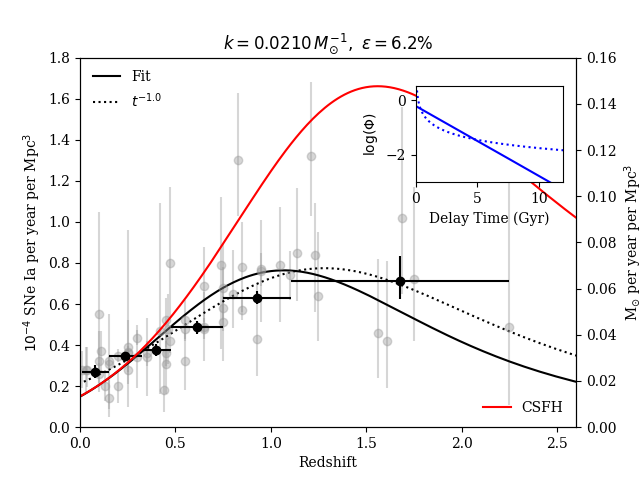
\includegraphics[width=6.5in]{figure_sfd_optimized} 
   \caption{\footnotesize In addition to rate values shown in previous figures, the $R_{\rm Ia}(z)$ model results of from optimal parameter fitting of the unimodal $\Phi(\tau)$ model is shown (solid black line) in comparison to a $\beta=-1$ power-law $\Phi(\tau)$ (dashed black line). The inset shows the comparison of the two $\Phi(\tau)$ models. The CSFH is shown on in red, and along the secondary ordinate. }
   \label{fig:sfd_optimized_curvefit}
\end{figure}

While the optimization results a model that is broadly consistent with the $t^{-1}$ model, it is not directly possible to estimate errors on the best-fit parameters, or the range of validity in this maximum likelihood optimization method. A Markov chain Monte Carlo (MCMC) is better suited for that.


\subsection{The MCMC solution\label{sec:mcmc_sfd}}
Exploring the parameter space in an MCMC allows both confirmation of the optimized solution and an exploration of the range of validity. We use the affine-invariant MCMC ensemble sampler from {\tt emcee.py}~\citep{Foreman-Mackey:2013pd} using the same likelihood function as shown in Equation~\ref{eqn:lf}, and set our uniform priors as described by the bounds, as shown in the previous section, with the exception of evaluating $\ln \varepsilon$ to allow MCMC step sizes of order unity, and using the prior $ -10 < \ln \varepsilon < 0$. We then set 1,000 walkers to explore 10,000 steps, for a total of 10 million iterations, the first 100,000 of which we discard as `burn-in'. The results of which are shown in Figure~\ref{fig:mcmc_sfd} and Table~\ref{tab:results}.


\begin{figure}[t] %  figure placement: here, top, bottom, or page
   \centering
   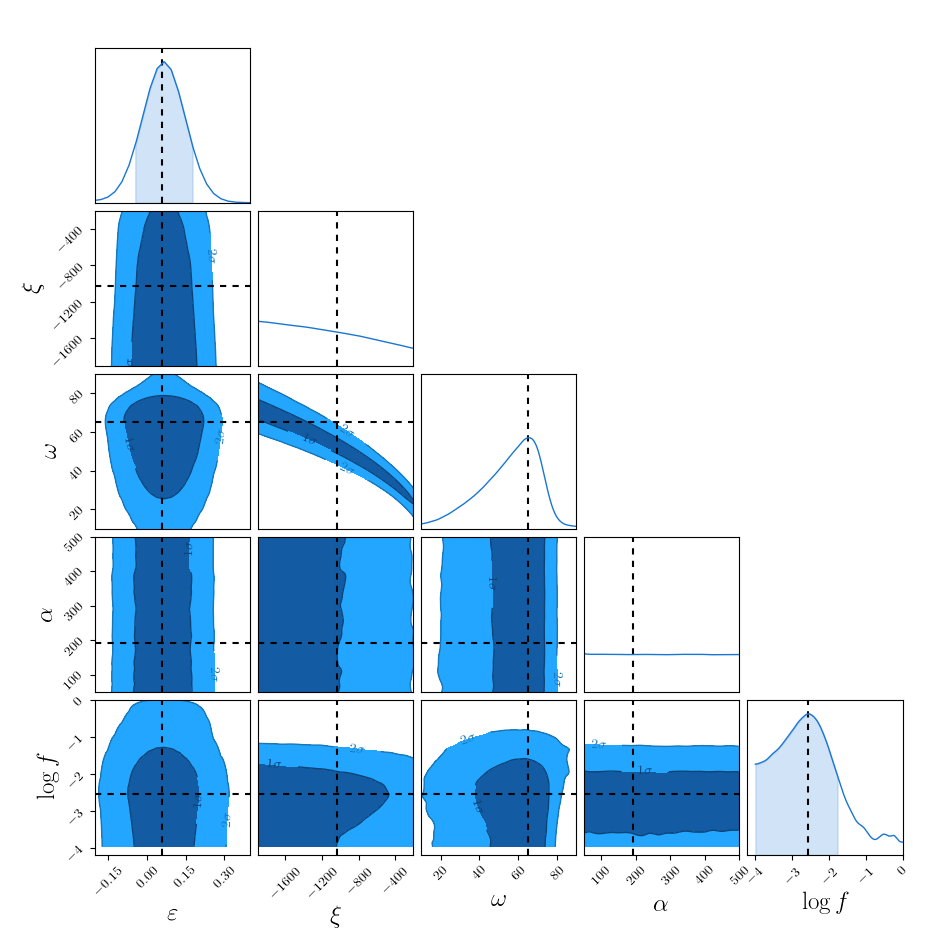
\includegraphics[width=6.5in]{figure_sfd_corners} 
   \caption{\footnotesize MCMC results on the parameters of a unimodal delay-time distribution model, fit to volumetric rate data and CSFH. Dashed lines indicate the maximum likelihood values. The $1-\sigma$ and $2-\sigma$ regions about those best fits are shown in dark and light blue, respectively. The plot generated using {\tt ChainConsumer.py} \citep{Hinton:2016qy}.}
   \label{fig:mcmc_sfd}
\end{figure}
\clearpage

\begin{figure}[t] %  figure placement: here, top, bottom, or page
   \centering
   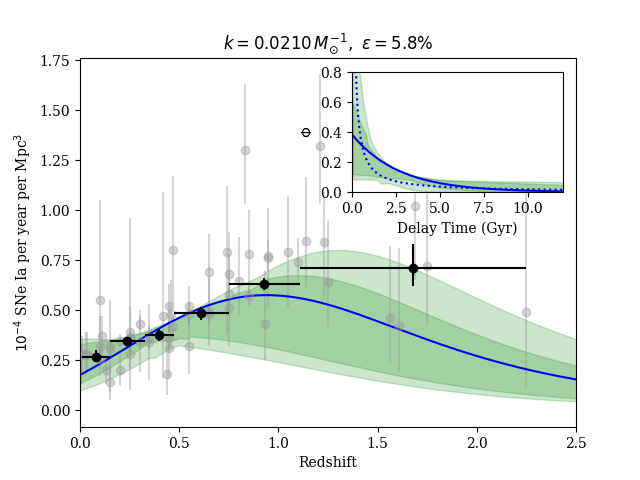
\includegraphics[width=6.5in]{figure_fit_demo_werr} 
   \caption{\footnotesize Similar to Figure~\ref{fig:sfd_optimized_curvefit}, the $R_{\rm Ia}(z)$ result of from MCMC best-fit is shown (blue line), with the 68\% and 95\% confidence intevals, in dark and light green, respectively. }
   \label{fig:figure_fit_demo_werr}
\end{figure}

As these result show, there is a clear convergence in $\ln f$, the factor by which reported statistical errors in rate measures are underestimated. It seems that nearly all values are underestimated from as little as 4\% to as much as 17\%, with most only about $7-9\%$ underestimated. So, while there is a large dispersion in rate values, these values are reasonably consistent with statistical errors, which are not grossly underestimated. Also fairly well constrained is the fraction $\varepsilon$, where only $6.0^{+0.3}_{-0.3}\%$ of WD stars contribute as SN~Ia progenitors. However, the parameters we wished to know the most about,  $\xi$, $\omega$, and $\alpha$, appear very much less constrained by the MCMC. There is a clear peak around $\omega\approx60$, but that value is also highly degenerate with the value of $\xi$.  There does not appear to be any convergence or preference in the value of $\alpha$.


While this does not seem to show a clear preference for a very specific parameterization the model, it does indicate a specific family of solutions that are related. With highly negative locations and broad widths, only the exponential-like tail of the distributions fall in the positive time space. As shown in Figure~\ref{fig:figure_fit_demo_werr}, the 68\% confidence interval about the best fit parameters, all indicate a rather flat DTD. \textcolor{red}{I should at least talk about Parallel-Tempering Ensemble MCMC, and perhaps Dynamic Nested Sampling}

\section{Delay Time Distributions from Star Formation Histories}
This is an evaluation of the maximum likelihood delay time distribution following the prescription of \cite{Maoz:2012a} but performed on the GOODS/CANDELS galaxies. For this analysis we use star formation histories derived using the Bayesian modeling approach of \cite{Pacifici:2012ve}. In summary, the galaxy physical properties are retrieved from a combined analysis of stellar and nebular emission utilizing an extensive library of star formation and chemical enrichment histories. These libraries build a large repository of rest-frame galaxy spectral energy distributions, which are then used to determine likelihood distributions of physical parameters from a Bayesian analysis of observed spectral energy distributions. This is method has been applied to the HST/WFC3-F160W-selected CANDELS catalogs for the GOODS-South \citep{Guo:2013rp}, and the GOODS-North \textcolor{red}{(Barro et al. , in preparation)}, into SFH catalogs~\cite[cf. ][]{Pacifici:2016ul}. We adopt only the median derived SFH of each galaxy for simplicity in this analysis.

For a given galaxy, the rate history of SNe~Ia per year ($r_i$) would be:
\begin{equation}
r_i (t) = h^2\,k\,\varepsilon\, \int_0^t \Psi_i(t')\,\Phi(\tau-t')\,dt',
\label{eqn:rate_history}
\end{equation}
\noindent where $\Psi_i$ is the star formation history of the galaxy (mapped in look-forward time), and $\Phi$ is the global delay time distribution model, also in look-forward time. The product of the rate at the observed epoch ($r_{i,0}$) and the observed control time ($t'_{c, i}$) of the galaxy-- which contains all the information on the temporal sampling and depth of the survey--  give ($m_i$) the expected number of observed SN~Ia events over the duration of the survey, or
\begin{equation}
m_i = r_i \, t'_{c, i}.
\end{equation}
\noindent The probability distribution of those observed events is likely Poisson, where of catching $n_i$ SNe~Ia from that galaxy when $m_i$ are expected is
\begin{equation}
P(n_i | m_i) = \frac{m_i^{n_i}e^{-m_i}}{n_i!}.
\end{equation}
\noindent The product of probabilities for all galaxies in the survey would then serve as the likelihood of a given delay-time distribution model. The log-likelihood, convenient for MCMCs, is then expressed by:
\begin{equation}
L = \prod _i^N P(n_i|M_i) \Rightarrow \ln L = -\sum^N m_i+\sum^N\ln\biggl(\frac{m_i^{n_i}}{n_i!}\biggr)
\end{equation}
\noindent in which the last term is zero for the galaxies which did not host SNe~Ia during the survey.\textcolor{red}{I should mention reference to the control times}.

\begin{figure}[t] %  figure placement: here, top, bottom, or page
   \centering
   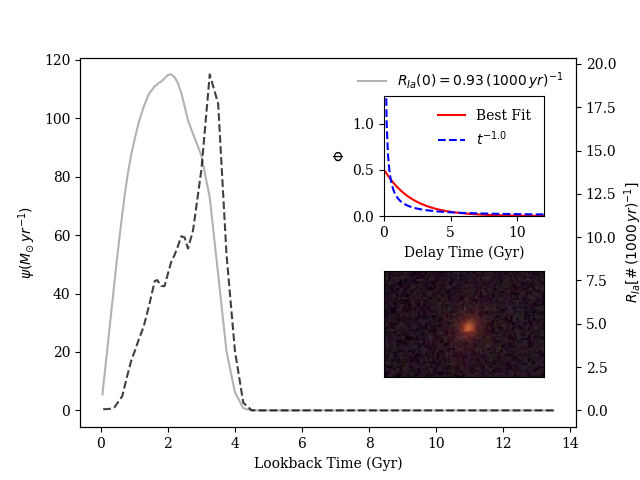
\includegraphics[width=3in]{figure_sfh_demo_v1} 
   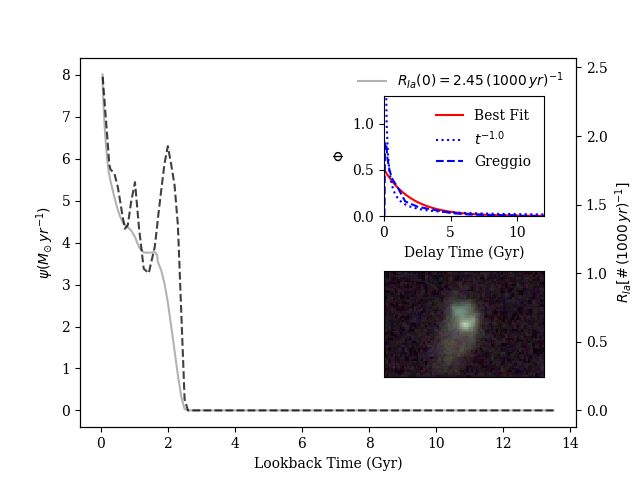
\includegraphics[width=3in]{figure_sfh_demo_v2} 
   \caption{\footnotesize Example star formation histories (dashed-line and left ordinate), and the resultant SN Ia rate histories (dotted-line and right ordinate) for two SN Ia host galaxies in our sample, SNe 2002hp (left) and 2003dy (right), in the GOODS-South and GOODS-North fields, respectively. Insets show the delay time distribution applied (upper right, in red) compared to $t^{-1}$ (blue dashed), and a three-color HST ACS/WFC image (lower right) of the SN host galaxy.}
   \label{fig:figure_sfh_fit_demo}
\end{figure}

Figure~\ref{fig:figure_sfh_fit_demo} shows examples ``SN~Ia rate history'' one would derive from Equation~\ref{eqn:rate_history} using the best-fit model from the MCMC on CSFHs, done in the previous sections. The figure shows star-formation histories for two SN Ia host galaxies, for SN 2002hp and SN 2003dy, respectively \cite[see][ for further details on these events]{Strolger:2004}. Both events are at $z\approx 1.3$, and in the GOODS-South and GOODS-North fields, respectively. The host of SN~2002hp is, however, a fast-forming/slow-quenching passive galaxy that underwent a very large burst of star formation just a few Gyr ago, that when convolved with the applied delay time distribution results in a relatively large expected rate of 0.93 SNe Ia per millennium at the observed epoch.  Conversely, the host of SN~2003dy is actively star forming but at a more modest rate, and has been doing so over the last few Gyr, resulting in a SN Ia rate at the observed epoch about three times larger, at 2.94 per millennium. Most non-hosts have predicted SN Ia rates at their observed epochs several orders of magnitude smaller than these two example hosts. 
  
There are 34 events we classified as SNe~Ia in the GOODS-South field, and 39 in the North field \citep{Strolger:2004, Dahlen:2008, Rodney:2014fj}, all but 6 of which were matched to a host galaxy in the SFH catalog. Two of these were rejected as the events spectroscopic redshifts were very inconsistent with the SFH catalog redshifts, and the other 4 were simply not in the SFH catalog, as they were either too faint or near the field edge to be listed in the composite photometry catalogs. 

\begin{figure}[t] %  figure placement: here, top, bottom, or page
   \centering
   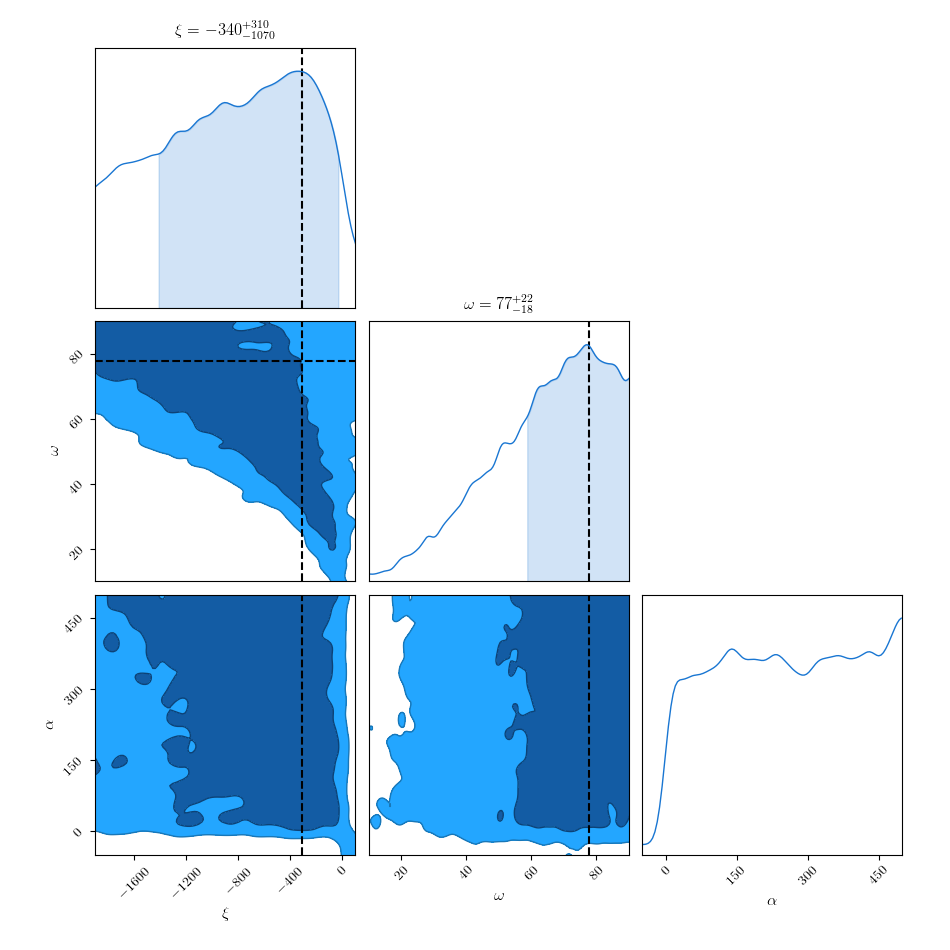
\includegraphics[width=6.5in]{figure_sfh_corners} 
   \caption{\footnotesize MCMC results on unimodal delay-time distribution model, fit to SFHs for 33,678 galaxies in the GOODS fields, 67 of which are SN~Ia hosts.}
   \label{fig:mcmc_sfh}
\end{figure}

The model parameters, $\xi$, $\omega$, and $\alpha$ are then explorable via {\tt emcee.py}. We keep the same uniform priors as bounds, as described in Sections~\ref{sec:optimized_soln} and \ref{sec:mcmc_sfd}. We fix the fraction $\varepsilon=0.06$ for convenience, and set 100 walkers exploring 500 steps on these parameters, the results of which are shown in Table~\ref{tab:results}.
\begin{table}[h]
    \centering
    \caption{Results for unimodal model}
    \label{tab:results}
    \begin{tabular}{cccccc}
        \hline
                Model test & $\ln \varepsilon$ & $\xi$ & $\omega$ & $\alpha$ & $\ln f$ \\ 
                \hline
		CSFH Max.~Likelihood (Optimized)&$-2.78$&$-1518$& $51$& $50$& $-2.41$\\
                CSFH MCMC & $-2.81^{+0.05}_{-0.05}$ & $-1258^{+523}_{-669}$ &$59^{+18}_{-12}$& $248^{+169}_{-171}$&  $-2.6^{+0.8}_{-0.7}$\\
                SFH MCMC & \nodata & $-1087^{+561}_{-604}$ &$73^{+22}_{-17}$& $242^{+168}_{-173}$&  \nodata\\
                \hline
    \end{tabular}
\end{table}




\section{discussion}
All three methods point to a family of delay-time distribution models that are somewhat similar to power-law models, but are more exponential, having much fewer prompt events in the 40 Myr to 1 Gyr range. The model also helps to clarify a discussion of 'prompt' vs 'delayed' progenitor mechanism. 

It is useful to evaluate the SN Ia rate that would result from the average galaxy (approx. $10^{10}$ M$_{\odot}$), undergoing a single, 1 M$_{\odot}$ yr$^{-1}$ burst of star formation, and the number of SNe Ia per year that would result over time. Figure~\ref{fig:logsnrate} shows the DTDs recovered in various time bins from Sloan galaxy data~\cite{Maoz:2010a, Maoz:2011, Maoz:2012a,Graur:2013} along with the derived power-law DTD models for field and galaxy cluster hosts. Rather than suggesting different power-law slopes, our best-fit DTD connects the data in clustered and field environments. 


The Hubble-time integrated SN Ia production efficiency, combining the $k$ and $\varepsilon$ terms, yields $N/M_{\star}=1.26$ events per 1000 M$_{\odot}$ formed.


\begin{figure}[t] %  figure placement: here, top, bottom, or page
   \centering
   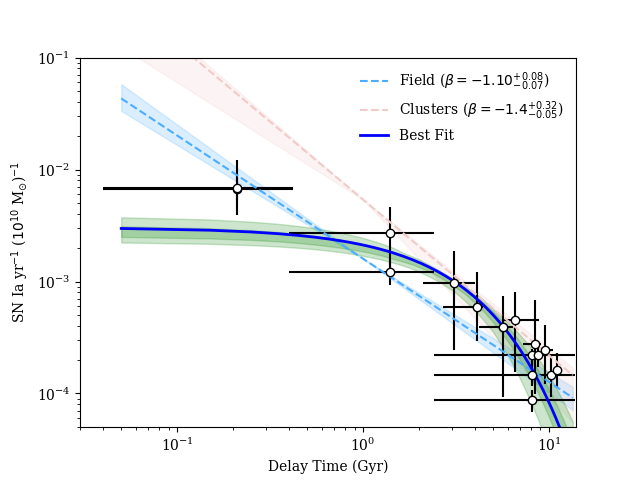
\includegraphics[width=6.5in]{figure_loglog_dtd}
   \caption{\footnotesize }
   \label{fig:logsnrate}
\end{figure}

\bibliography{strolger}{}
%
%\begin{table}
%    \centering
%    \caption{Parameter Covariance MCMC SFD}
%    \label{tab:parameter_covariance}
%    \begin{tabular}{c|ccccc}
%         & $f$ & $\xi$ & $\omega$ & $\alpha$ & $\log \phi$\\ 
%        \hline
%              $f$ &  0.41 & -125.69 &  6.61 & 33.98 & -0.41 \\ 
%            $\xi$ & -125.69 & 412816.10 & -14898.10 & -52398.20 & 518.74 \\ 
%         $\omega$ &  6.61 & -14898.10 & 660.60 & 2209.32 & -22.89 \\ 
%         $\alpha$ & 33.98 & -52398.20 & 2209.32 & 27290.24 & -131.67 \\ 
%        $\log \phi$ & -0.41 & 518.74 & -22.89 & -131.67 &  2.35 \\ 
%        \hline
%    \end{tabular}
%\end{table}


\end{document}